This study showed, that each of two approaches has its own use cases. Blockchain is particularly good in removing third party-related trust issues, which is present in vast majority of centralized systems. Usage of a blockchain is also very beneficial, when it comes to the question of availability and data integrity. Its high degree of data integrity is achieved by strong cryptographic bonds between the blocks.

\begin{figure}[H]
\centering
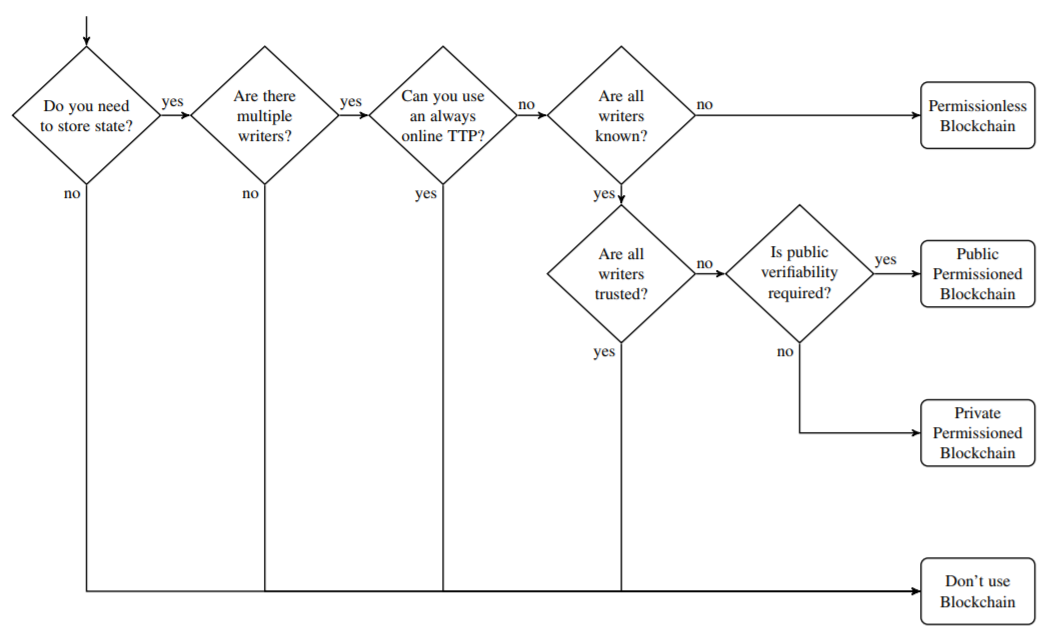
\includegraphics[scale=0.54]{images/blockchainusecase.png}
\caption{Flowchart, describing if a blockchain should be used \textnormal{\citep{wust2017you}}. TTP stands for "trusted third party".}
\label{fig:blockchainuse}
\end{figure}

When considering a particular use case of Blocket Secure Package, usage of blockchain may seem like a good idea, if the flowchart in Figure \ref{fig:blockchainuse} is taken into consideration.

\begin{description}
\item[Do you need to store state?] 
Yes. The state in this service is the money being transfered and any information about the delivery (sensor data for example).
\item[Are there multiple writers?]
Yes. Buyers, sellers and sensors are all writers.
\item[Can you use an always online TTP?] No. As was established in the analysis, there are potential trust related issues, regarding Blocket, as a central authority.
\item[Are all writers known?] No. Anyone can be a buyer and seller in this system.
\end{description}

However, usage of blockchain as a backend puts enormous constraints on some aspects of the Secure Package system. Those constraints are mostly associated with large gas consumption and had to be addressed by prioritizing some modules of the system over other less important ones. By far the biggest concerns, regarding a full-on blockchain implementation, are its ridiculous storage cost, impracticality of performing frequent smart contract function calls and unpredictable latency.

The main point, that this study brought up is that there is no solution, which generally is better. It all depends on what aspects and features are more and less important to the user. If user-friendliness of an all-in-one web marketplace, which is cheap to use, does not have a significant bottleneck on transaction density and storage, and does have a degree of transparency, is desirable for a user, then the centralized version is a good choice. On the other hand, if a high degree of privacy, absence of third party and high degree of trust is important, the decentralized blockchain-based system would be a better option.

As a result of all the discussions, statements and studies of this thesis work, a conclusion can be drawn. In order to implement a system, that does not posses any specific approach-related drawbacks, the best solution would be to combine those two technologies. In order to do that, modules of the Secure Package, or any other application, can be categorized during the design phase, according to their demands and specific requirements. Modules, which require high degree of trust and privacy may be handled by a blockchain, while modules, that process large amounts of interactions with the backend and require high amounts of storage space may be handled by a database server.

Another option would be to use the Ethereum blockchain as a verification mechanism behind a centralized backend with a database server. This could potentially be achieved by recording all changes, made to the database contents (using roughly the same principal, as blockchain transactions), and storing the hashes of those changes in a blockchain. Those hashes could later be associated with a specific agreement identifier, thus making tracing of changes possible.

Going back to the Section \ref{section:purpose}, the questions, which were displayed at the end of the section, can now be answered.

\begin{itemize}
\item \textit{"Is it possible to create a centralized system, that doesn't use a blockchain, but possesses its advantages without having its blockchain-specific drawbacks?"} - Partially yes. A centralized system can be implemented with transparency and anonymity in mind. However, the trust-related issues can not be completely addressed, if a third party is involved in any degree. In order completely to get rid of the party, in most cases, a blockchain is the way to go.

\item \textit{"Can blockchain-specific features improve a centralized system and address some of its issues without a need for drastic architecture changes?"} - Yes. Introduction of some blockchain-specific features does not require any additional hardware. Assuming, that a centralized application is built with reusability and modifiability in mind, it could easily be extended to possess higher degree of transparency, anonymity and privacy.
\end{itemize}




